\begin{figure}
\centering

\begin{subfigure}{\linewidth}
\centering
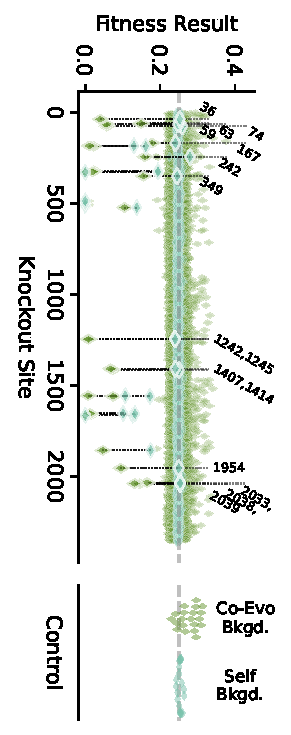
\includegraphics[height=0.9\linewidth,angle=90]{binder-2026-06-22-eco-gwas.ipynb/binder/teeplots/viz=subplots+ext=.pdf}

\caption{\footnotesize TODO}
\label{fig:ecogwas:sites}
\end{subfigure}

\vspace{1ex}

\begin{subfigure}{\linewidth}
\centering

\includegraphics[height=0.35\linewidth]{binder-2026-08-13-eco-gwas-weakstrong.ipynb/binder/teeplots/2026-08-13-eco-gwas-weakstrong/col=classification+hue=classification+style=classification+viz=relplot+x=focal-prevalence-backgroundbb+y=focal-prevalence-focalbb+ythresh=0.45+ext=.pdf}%

\includegraphics[height=0.35\linewidth]{binder-2026-08-13-eco-gwas-weakstrong.ipynb/binder/teeplots/2026-08-13-eco-gwas-weakstrong/color=white+viz=boxplot+x=classification+y=count+ythresh=0.45+ext=.pdf}

\caption{\footnotesize TODO}
\label{fig:ecogwas:ythresh045}
\end{subfigure}

% https://github.com/mmore500/oee4/blob/34f2116c799c849f329e91f544e57daa23eff9da/binder/2026-06-22-eco-gwas.ipynb
% https://github.com/mmore500/oee4/blob/34f2116c799c849f329e91f544e57daa23eff9da/binder/2026-08-13-eco-gwas-weakstrong.ipynb
\caption{%
\textbf{Case study strain selects for genotype complexity in co-evolved partner.}
\footnotesize
In stint-100 isolate of case study background strain, 14 genome sites exhibited strong adaptive benefit compared to single-site knockouts when tested with case study strain absent.
However, with case study strain present, adaptive benefit was detected at an additional 18 genome sites.
Co-evolutionary adaptation to case study strain thus accounts for 56\% (18/32) of detected genotype complexity in background strain.
TODO
}
\label{fig:ecogwas}
\end{figure}
